\section{The \lhcb detector}

The \lhcb detector is a single arm forward spectrometer, reminiscent of a fixed target experiment,
because \bbbar pairs are predominantly produced with momentum vectors close to the beam line in
partonic interactions.
Figure~\ref{fig:lhcb:bbbar} shows the number of \bquark and \bquarkbar quarks produced in bins of
this angle; the acceptance of \lhcb covers approximately $25\,\%$ of \bbbar pairs, this is also indicated.
Using the coordinate system where $z$ is defined by the \lhc beam pipe,
%($z=0$ being the interaction point),
\lhcb has an acceptance in pseudorapidity, $\eta$, of $1.8<\eta<4.9$.  %(\lesssim)
Pseudorapidity is defined as $-\log\left(\tan\tfrac\theta2\right)$, where $\theta$ is the angle
between the $z$ axis and the momentum vector of some particle emerging from the interaction point.
The interaction point is at $z=0$ and the positive $z$ direction is referred to as downstream.
The $x$ and $y$ axes are then defined by the horizontal and vertical directions respectively.
Figure~\ref{fig:lhcb:lhcb} is a schematic diagram of the \lhcb indicating the coordinate system and
subdetectors.
A schematic diagram of the \lhcb detector is shown in Fig~\ref{fig:lhcb:lhcb}.

\begin{figure}
  \begin{center}
    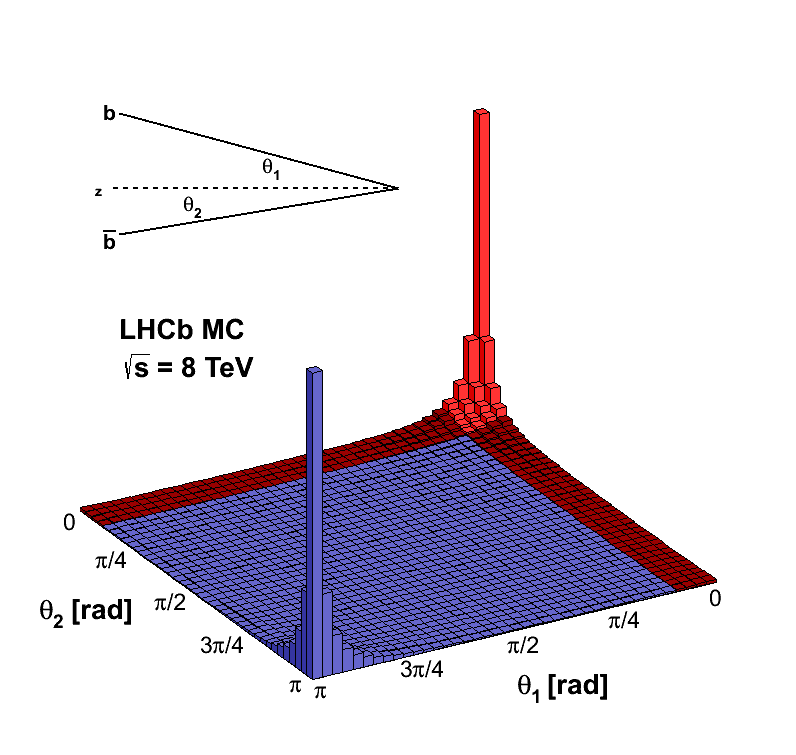
\includegraphics[width=0.5\textwidth]{acceptance}
  \end{center}
  \caption[Simulated production of \protect\bbbar pairs]
  {\small
    Simulation of the production of \bquark and \protect\bquarkbar quarks with angles $\theta_1$ and
    $\theta_2$ from the beam axis respectively.
    The dark red areas indicate those quarks which fall within the \lhcb acceptance, the light red
    area therefore is all \bbbar pairs within the acceptance.
  }
  \label{fig:lhcb:bbbar}
\end{figure}

\begin{figure}
  \begin{center}
    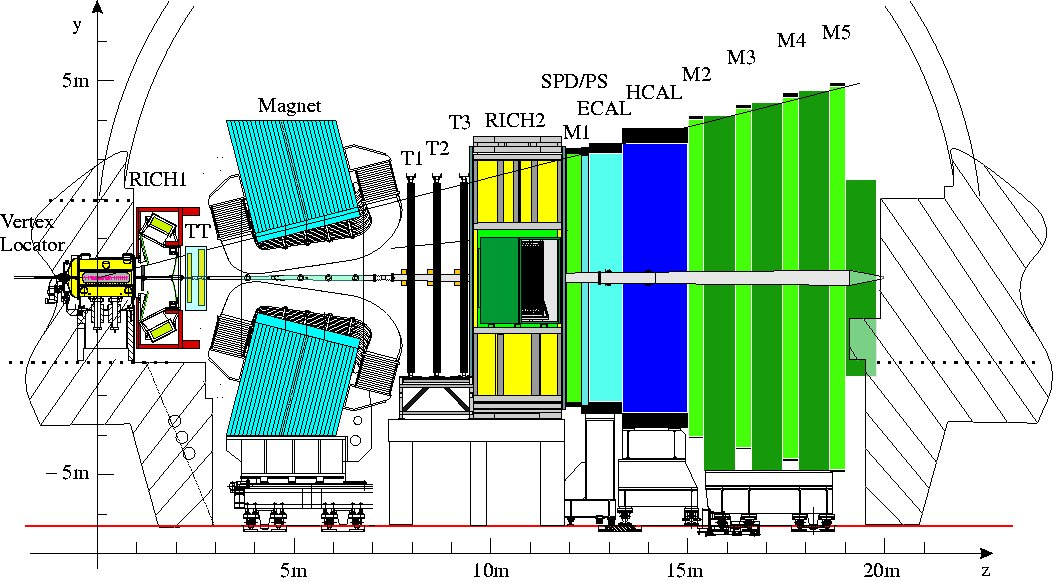
\includegraphics[width=\textwidth]{LHCb_detector}
  \end{center}
  \caption[\lhcb detector]
  {\small
    Schematic diagram of the \lhcb detector with labeled subdetectors and coordinate system, the
    $x$ direction comes out of the page.
  }
  \label{fig:lhcb:lhcb}
\end{figure}

Spatial coordinates of charged particles traversing the detector are recorded as hits in the
tracking systems.
Particle momentum is deduced by their curvature in the $x$ direction when then pass through the
detector region which is immersed in a magnet field.
This field has an integrated strength of $4\,\mathrm{Tm}$ and is provided by a large conventional
magnet.
Other subdetector systems include two Cherenkov detectors used for particle identification;
calorimeters, which are used for triggering; and muon stations which are used for identifying and
triggering muons.



\subsection{Tracking}
Tracking begins with the \velo which precisely measures spatial
coordinates of charged particle close to the interaction point.
The \velo must be able to resolve all tracks and distinguish primary vertices (PVs) coming from
proton-proton interactions, and secondary vertices indicative of decays of heavy flavour.
For example, a \Bp hadron with a momentum of $100\gev$ will travel $\sim1\cm$ before decaying.
This must all be done in a high track multiplicity environment.

%This is a high multiplicity environment and it is important to correctly resolve each primary
%vertex from proton-proton collisions, and secondary vertices formed by the decay of a hadron
%containing a \bquark or \cquark.
%Particles containing a \bquark quark typically have a finite, non-zero, lifetime; for example a \Bp
%with a momentum of $100\gev$ will travel $\sim1\cm$ before decaying.
%Resolving these indicative secondary decay vertices in the high occupancy area surrounding the
%interaction point is therefore of vital importance to the \lhcb physics program.

The \velo subdetector is made up of 21 modules orientated in the $x-y$ plane.
Each module consists of two layers of silicon strip detectors measuring hits in $r$ and $\phi$
coordinates.
The pitch of the silicon strips vary from $\sim40\mum$ nearest the centre to $\sim100\mum$ at the
extremity.
To decrease the distance of extrapolation of tracks to vertices,
% increase spatial resolution of vertices,
the active area of the \velo starts $8\mm$ from the beam line.
This is made possible because each module is split into two halves which retract when the \lhc beam
is unstable.
Its design leads to a detector with high impact parameter resolution, which can detect tracks
emerging from a proton-proton interaction in the range $1.6<\eta<4.9$ and $|z|<10.6\cm$.
Figure~\ref{fig:lhcb:velo} shows the geometry of the \velo.

%Increased accuracy is achieved by reducing the distance of extrapolation for each track back to its
%vertex of origin.
%To do this, each module constitutes two halves which are separate during the fill and
%acceleration stages of the \lhc, but are then brought together such that the detection area begins
%8\mm from the beam axis.
%Each of the $r$ and $\phi$ layers is made up of silicon strips with increase in pitch from
%$\sim40\mum$ nearest the centre to $\sim100\mum$ at the extremity.
%charged particles in $r,\phi$ coordinates using separate layers within each module, a diagram of
%this arrangement is shown in Fig~.\ref{fig:lhcb:velo}

\begin{figure}
  \begin{center}
    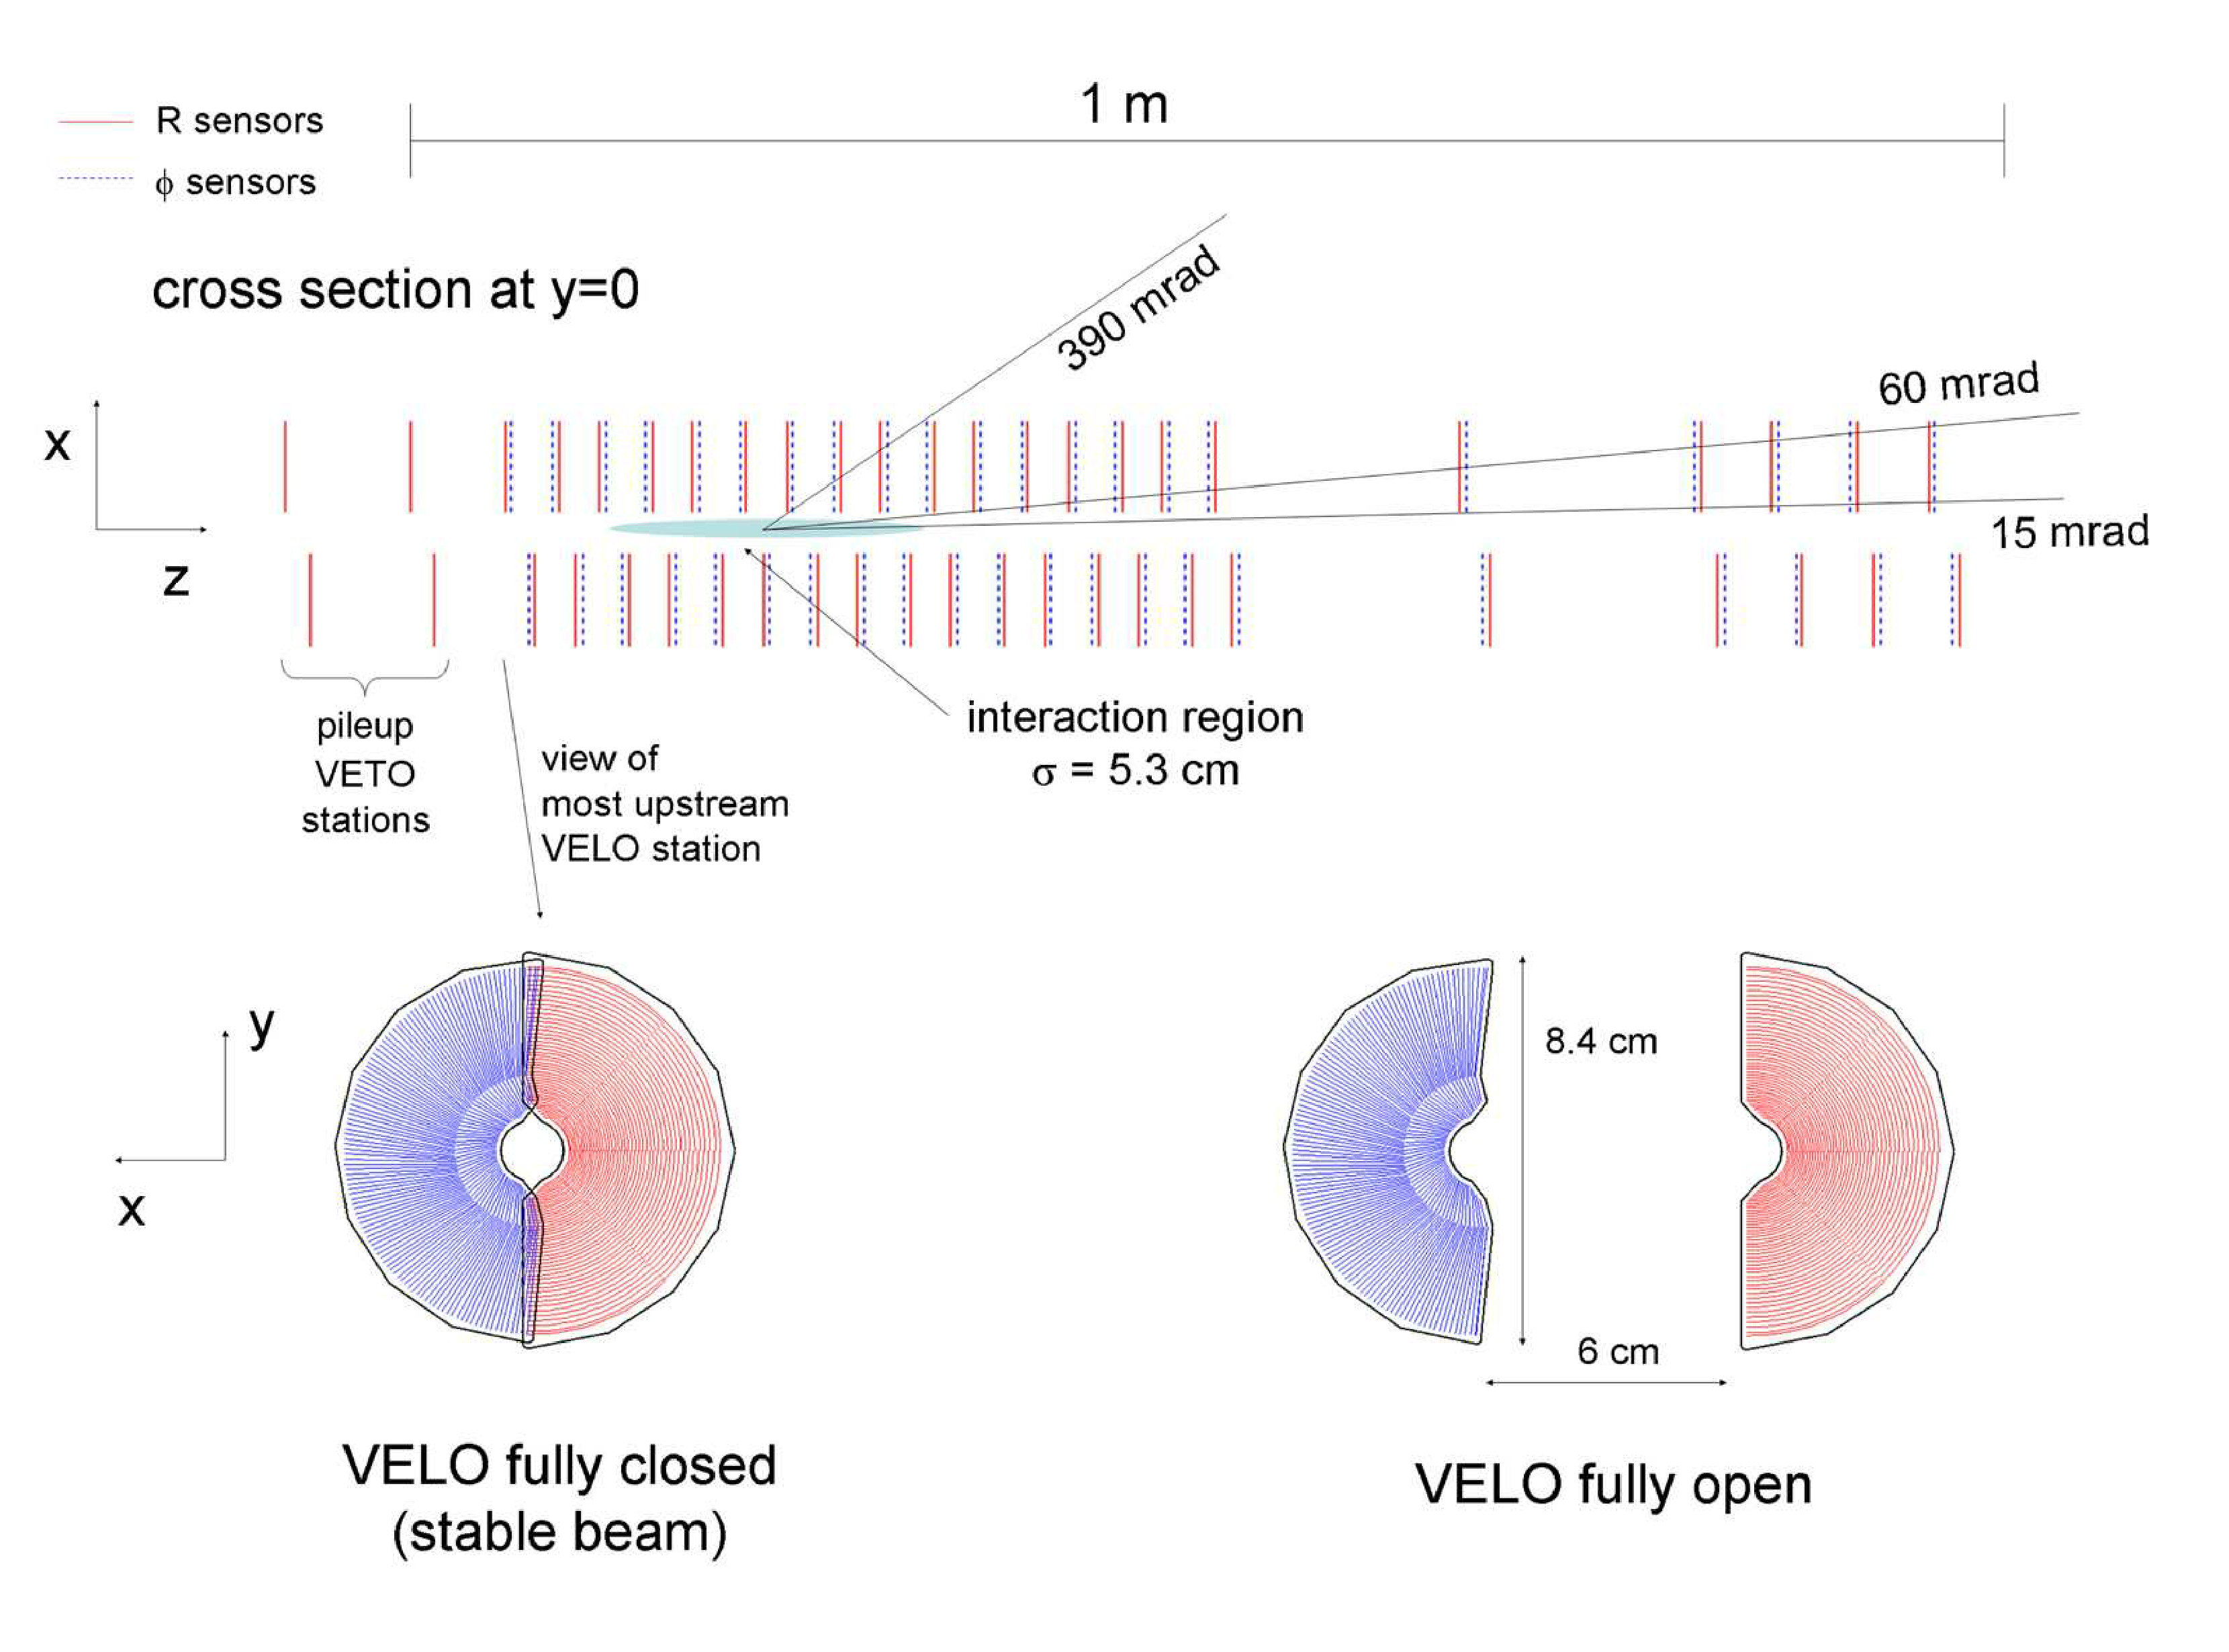
\includegraphics[width=0.7\textwidth]{velo}
  \end{center}
  \caption[\lhcb \velo]
  {\small
    The layout of silicon sensors the \velo in showing $r$ sensors in red and $\phi$ sensors in
    blue.
    A cross section at $y=0$ in the $x-z$ plane is shown while the \velo is closed.
    Along side these are slices in the $x-y$ plane, with the \velo closed and open.
  }
  \label{fig:lhcb:velo}
\end{figure}

There are four further tracking stations: the \ttracker, which sits directly
before the magnet; and the remaining three stations (T1-3), are immediately downstream of the
magnet.
Each tracker exhibits an $x-u-v-x$ geometry, where $u$ and $v$ are rotated by $-5^\circ$ and
$+5^\circ$ with respect to $y$.
Tracking stations T1-3 consist of a cross-shaped \intr, which is closest to the beam, and
an \ot covering the remaining area.
Together, the \ttracker and \intr form the Silicon Tracker (ST) which are silicon microstrip
detectors with a pitch of $200\mum$.
This gives the \st a single hit resolution of $50\mum$.
Each layer of the \ot is made of two layers of drift tubes with a diameter of $4.9\mm$, giving a
drift coordinate resolution of $200\mum$.
%while the \ot is fabricated of straw drift tubes.
In all the \velo, \st and \ot give the \lhcb detector excellent momentum resolution;
$\tfrac{\Delta p}{p}$ between 0.4 and 0.6\,\% for particles with momenta of $5\gev$ and $100\gev$
respectively.
%Essential for good resolution of the B invariant mass.


\subsection{Particle identification}
Beauty flavoured hadrons can decay into any (allowed) combination of hadrons and
leptons.
Misidentifying daughter particles when reconstructing a candidate $B$ hadron gives rise to a
combinatorial background making the signal less significant.
\lhcb can distinguish hadrons from one another using two \rich detectors, and penetrating muons are
identified by the muon system.


The \rich detectors work by focusing the Cherenkov light emitted by particles passing through
given materials, or radiators, onto photomultipliers using spherical mirrors.
The opening angle of the Cherenkov radiation cone, $\theta_\mathrm{Ch}$ is related to the
particle's phase velocity, $v_p$, via:
\begin{equation}
  %\cos\theta_\mathrm{Ch}=\frac1{n\beta}. %, \beta=\frac{v_p}{c}.
  \cos\theta_\mathrm{Ch}=\frac1{n\beta},\mathrm{\;where\;} \beta=\frac{v_p}{c}.
\end{equation}
With a measurement of the particle's momentum from the tracking system and only a few possible
masses (that of the electron, muon, pion, kaon or proton) likelihoods are constructed for each
track based on the ring of photons which such a particle would emit.
The measured quantity is that of the delta log-likelihood ($\Delta LL(X-\pi$), which is the difference between the
logarithm of the likelihood of the hypothesis of the particle $X$ compared to the null hypothesis of the
pion.

The two \rich detectors at \lhcb contain three different radiators (Aerogel and \cfourften in
\richone, and \cffour in \richtwo) allowing them to cover different momentum ranges.
\richone is situated immediately downstream of the \velo and covers the low momentum range,
$2<p<40\gev$, while \richtwo lies downstream of T3 and covers the range $15<p<100\gev$.
The variation of $\theta_\mathrm{Ch}$ on momentum for pions, kaons and protons is shown in
Fig.~\ref{fig:lhcb:pideff}.

In this way, the \lhcb detector can achieve excellent pion-kaon separation, for a kaon with
momentum around $20\gev$ the identification rate is near $100\,\%$ and the pion misidentification
rate is a few percent as shown in Fig.~\ref{fig:lhcb:pideff}.
%This figure also shows the variation of $\theta_\mathrm{Ch}$ with momentum for pions,
%kaons and protons; it also shows \lhcb's ability to discriminate between pions and kaons.

\begin{figure}
  \begin{center}
    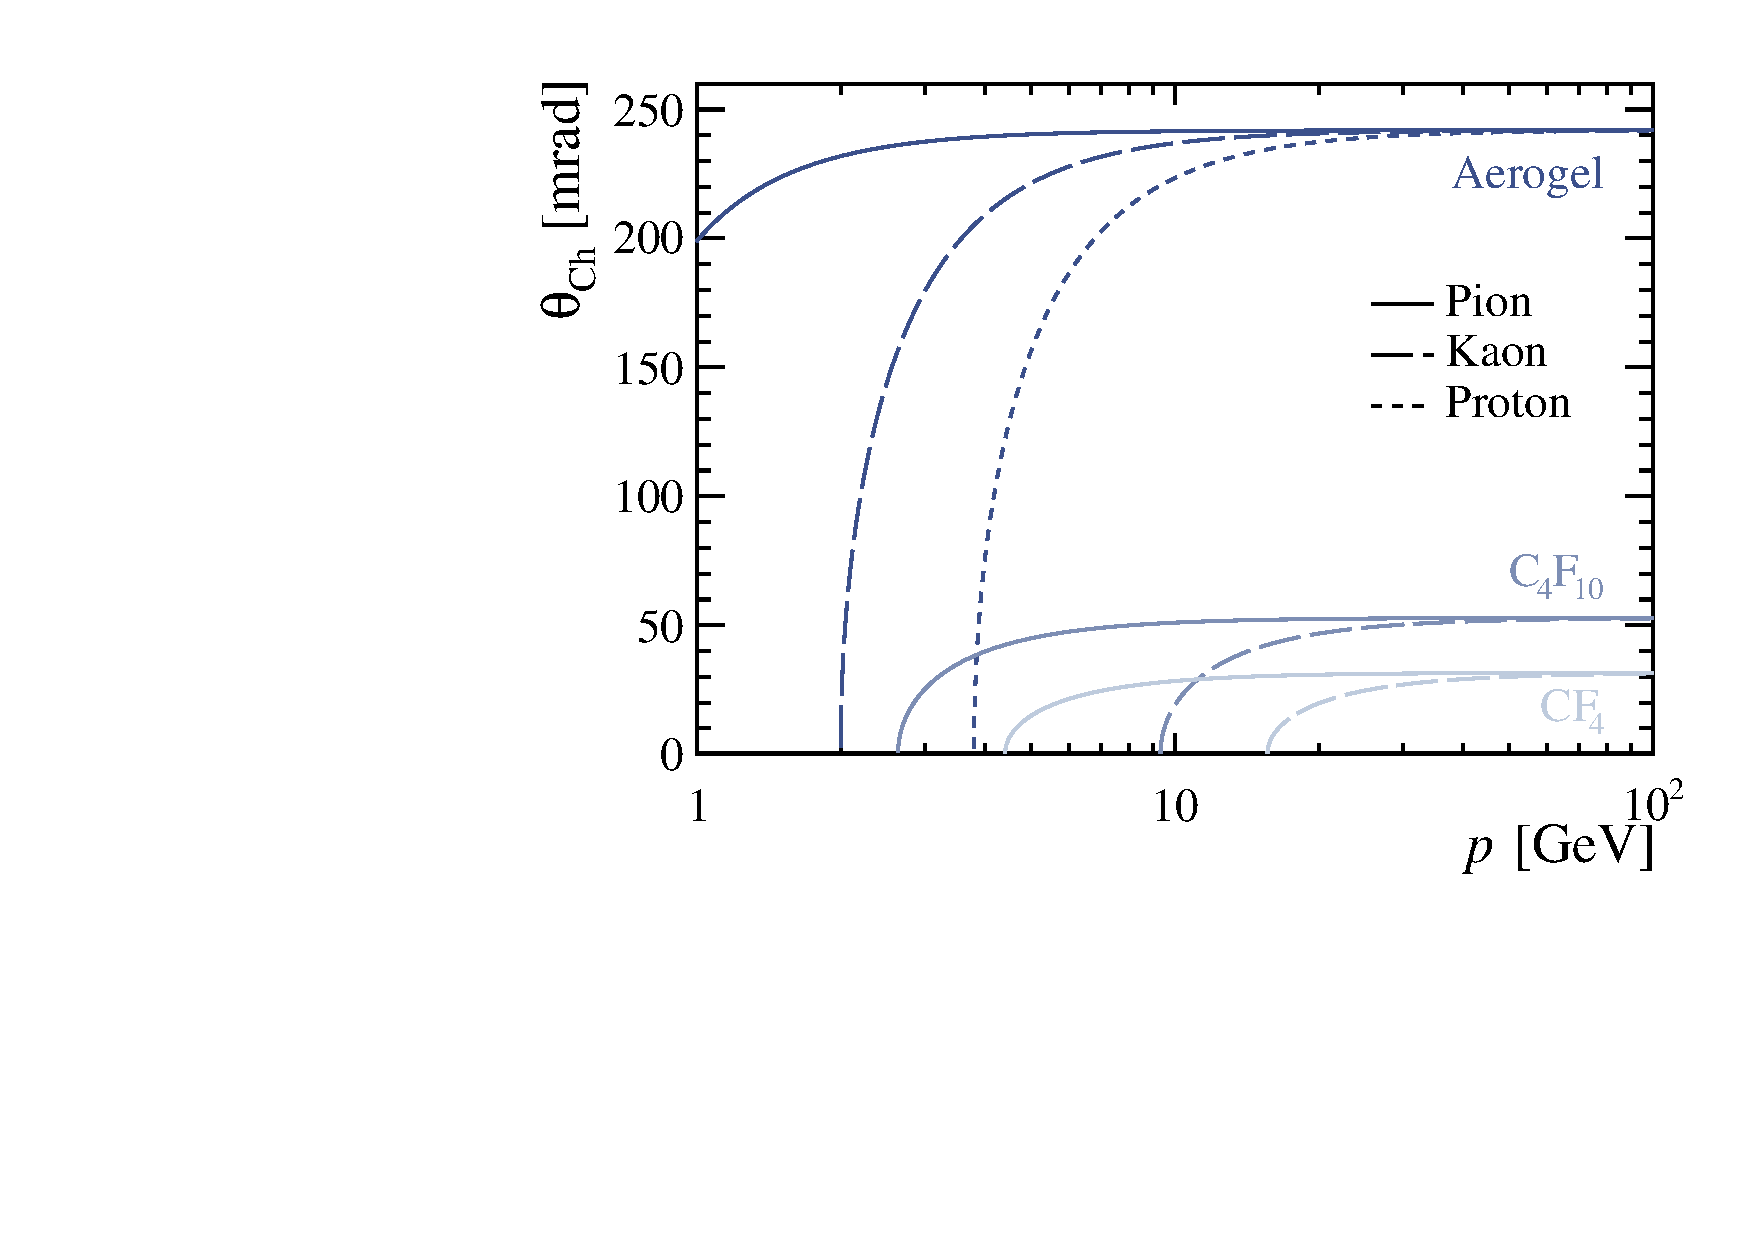
\includegraphics[height=0.2\textheight]{cherenkov_theory}
    %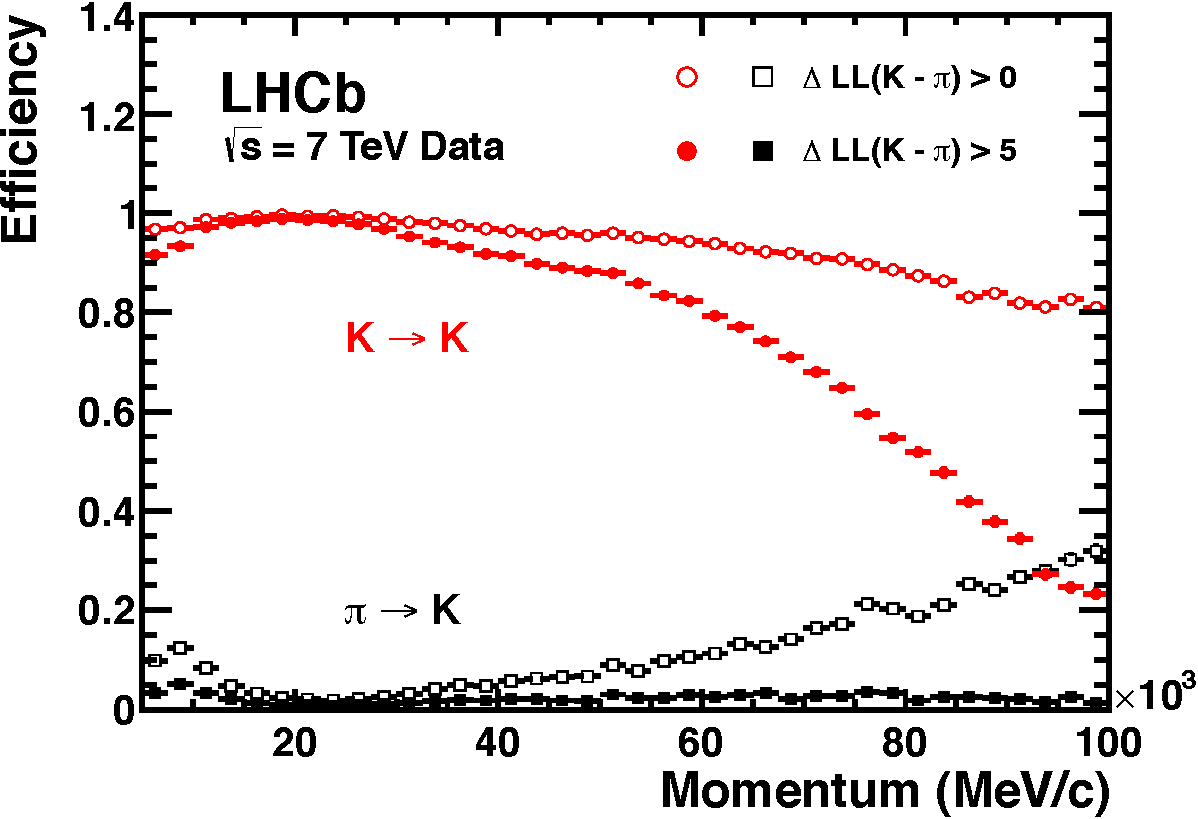
\includegraphics[height=0.2\textheight]{KandPi_2_K}
    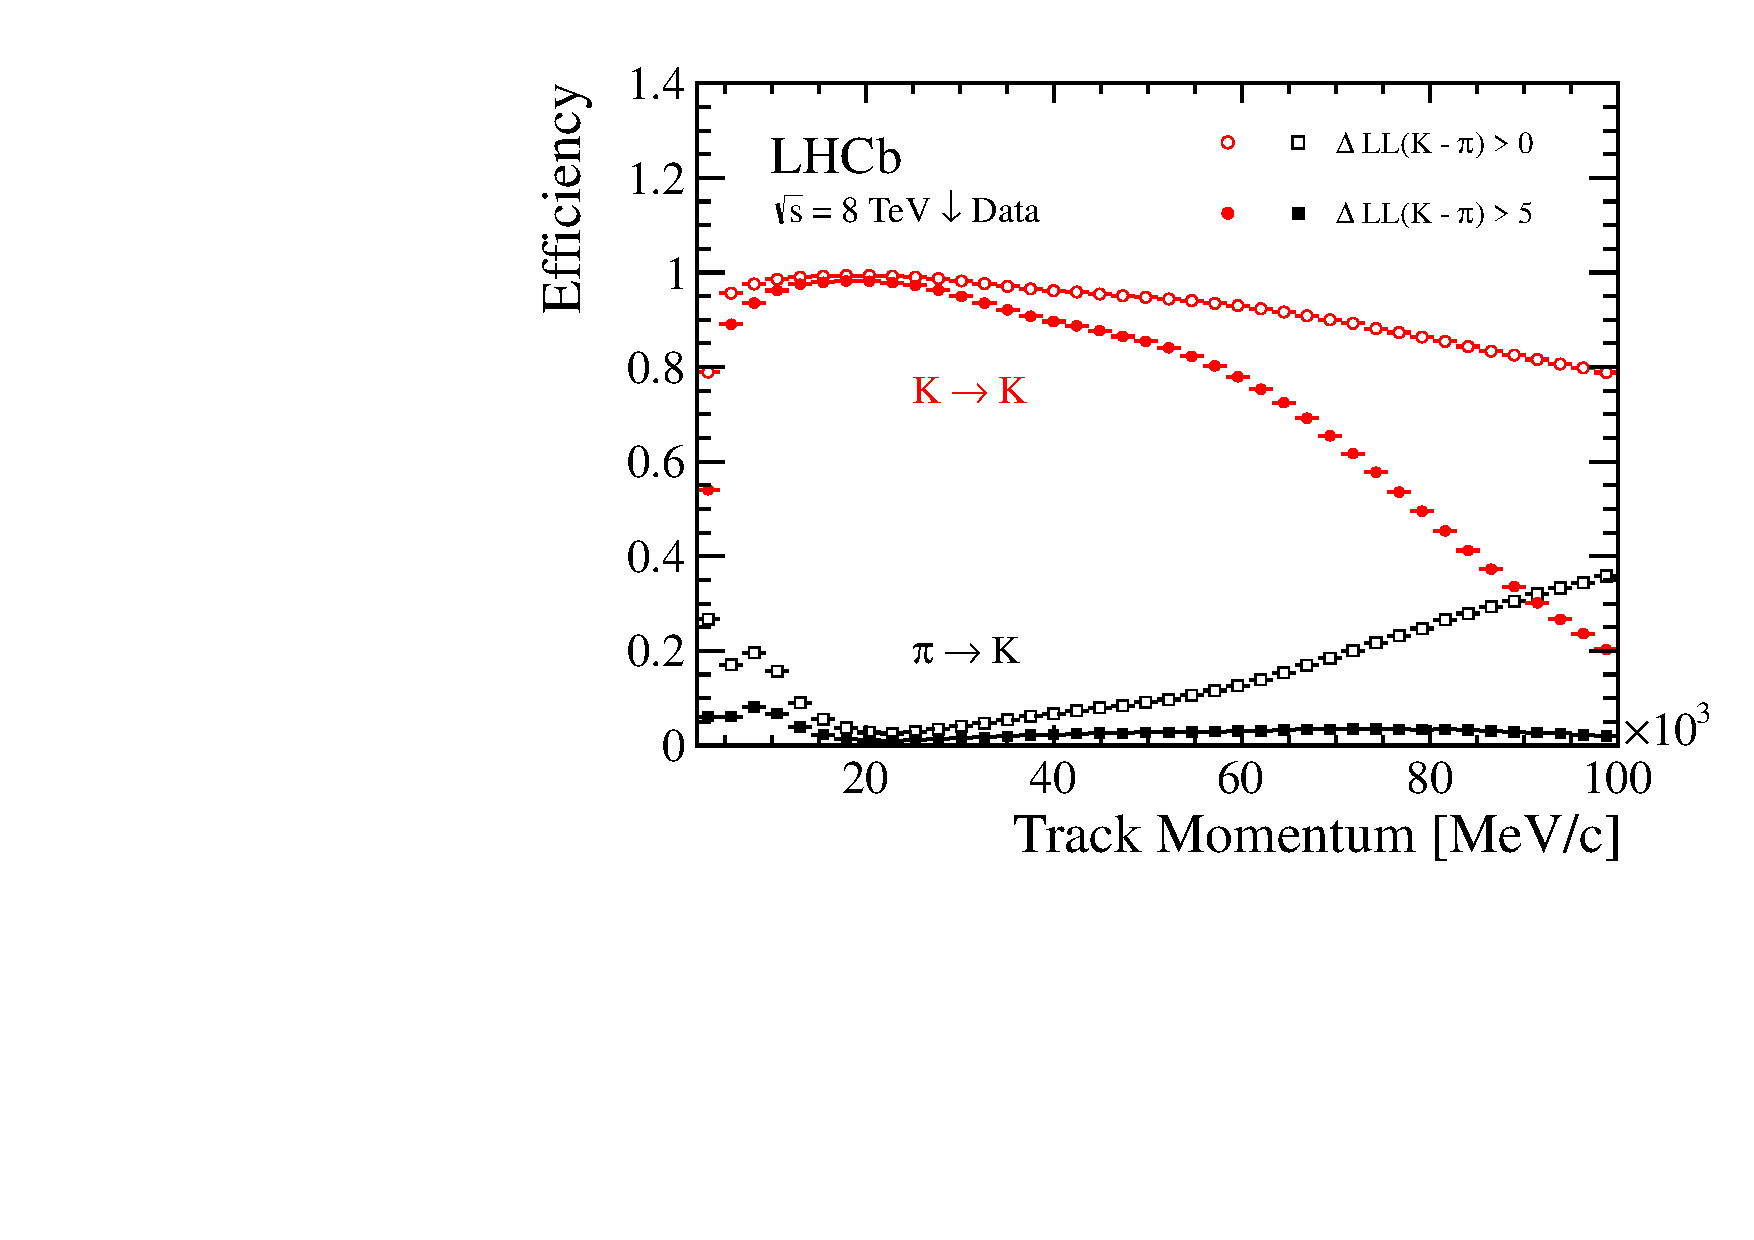
\includegraphics[height=0.2\textheight]{KPi_S20_MagDown_DLL}
  \end{center}
  \caption[Particle identification and Cherenkov angles]
  {\small
    Cherenkov angle as a function of momentum for pions, kaons and protons in the three different
    radiators (left), and the kaons-pion separation performance as a function of momentum, from
    Ref.~\cite{LHCb-DP-2012-003}.
  }
  \label{fig:lhcb:pideff}
\end{figure}

The detector systems downstream of \richtwo, namely the muon and calorimetry systems, are used for
\pid and in the trigger; triggering will be covered in the following section.
As discussed, the \rich detectors excel in hadron identification; for the identification of
electrons, photons and muons information from the five muon stations (M1-5) and calorimetry system
are used.
The calorimeters are situated between M1 and M2-5.

The general structure of the calorimetry system is that of an \ecal followed by an \hcal.
The \ecal is a shashlik detector, made of alternating layers of lead, reflector and scintillating
material, and the light is read out by photomultipliers.
This subdetector is 25 radiation lengths long to ensure that all electromagnetic energy is
deposited within before the \hcal.
It has an energy resolution of $\sigma_E/E = 10\%/\sqrt{E} \oplus 1\%$ where $E$ is in GeV.
Two additional subdetectors, the \spd and \presh, provide some particle identification at trigger
level, details of the trigger are provided later.
Showers caused by the interaction of electromagnetic particles interacting with a thin lead plate
are detected in the \presh.
Further upstream of the layer of lead is the \spd, which identifies charged tracks.
The \hcal consists of layers of iron and scintillating tiles which run parallel to oncoming
particles.
Each subdetector within the calorimetry system has increased cell density near the beam to cope
with higher track multiplicity in this region
Due to restrictions in space, the \hcal is only 5.6 nuclear interaction lengths long, and has a
resolution of $\sigma_E/E = (69\pm5)\%/\sqrt{E} \oplus (9\pm2)\%$, where $E$ is in GeV.


Finally, there is the muon system.
Each station uses Multi-Wire Projection Chambers exclusively, except for the centre of M1, where
the expected flux would age this technology too quickly; in this area Gas Electron Multiplier
detectors are used.
Like the calorimeters, the muon stations have increased cell density near the beam; however in
contrast, the cell density is greater in the bending plane than the non-bending plane in order to
increase momentum resolution.
Only muon stations M2-5 are used for particle identification; theses are interleaved with plates of
$80\cm$ thick lead plates, so only very energetic muons reach M5.
For this reason M4 and M5 are used to identify these penetrating muons, while M2 and M3 have
increased single hit resolution for momentum measurements.
In many \lhcb analyses a muon is identified based on hits within the muon system, the criteria is
known as {\tt isMuon}.
It is defined as follows: particles with momenta $3<p<6\gev$ must be associated with hits in M2 and M3; if
$6<p<10\gev$ there must be hits in M2, M3 and either M4 or M5; else if $p>10\gev$ there must be
associated hits in all M2-5.


\subsection{Trigger}
With a pp interaction rate of $40\mhz$ there is clearly too much information associated with an event
to write them all to disk.
Instead a multistage trigger is employed.
The first level trigger, \lone, is embedded in the hardware of \lhcb and is fully synchronous with
the bunch crossing rate.
It uses momentum and energy information to select events.
Its output rate is $1\mhz$.
Two software triggers are fast enough to perform tracking algorithms and use information from
multiple subdetectors to reduce the events written to disk to $5\khz$.
The flow of data through the trigger is shown in Fig.~\ref{fig:lhcb:trigger}.

\begin{figure}
  \begin{center}
    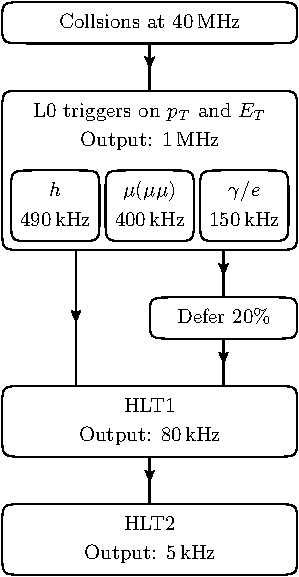
\includegraphics[scale=1]{trigger}
  \end{center}
  \caption[Trigger sequence]
  {\small
    The flow of the \lhcb trigger system in 2012.
  }
  \label{fig:lhcb:trigger}
\end{figure}

There are five \lone trigger lines; one each for photons, electrons, hadrons, muons and dimuons.
The decisions of the former three are based on calorimeter information while th others use muon
system information.
A cluster in the \ecal and \hcal is defined as two-by-two calorimeter cells.
For each cluster the transverse energy, $E_T$, is calculated:
\begin{equation}
  E_T = \sum_{i=1}^4E_i\sin\theta_i,
\end{equation}
where $E_i$ is the energy in cluster $i$ and $\theta_i$ is the angle between the average
interaction point and the cell's centre.
These clusters are then categorized as follows.
A hadron candidate is the largest $E_T$ cluster in the \hcal summed with the $E_T$ of the \ecal
cluster in front, if there is one.
A candidate photon (electron) is the largest $E_T$ deposit with hits in the \presh cells in front and
no hits (at least one hits) in the nearest \spd cells.
The $E_T$ of each candidate is compared to thresholds, and the event is retained if one or more is
exceeded.

First level trigger lines associated with muons base their acceptance on measurements of \pt.
Each quadrant of the muon system is read out independently, so muons which cross boundaries cannot
be triggered.
The muon candidates with the highest and second highest \pt are selected by each quadrant by
searching for straight lines through M1-5 in the $z-y$ plane, and in the $z-x$ plane if
$p_T>0.5\gev$.
The M1 station is used here to increase the \pt resolution of tracks, this enables (without the
tracking information) a resolution of about $25\,\%$ of fully reconstructed tracks.
Events are accepted based on candidates from all quadrants with values of $p_T^\mathrm{max}$ and
$p_T^\mathrm{max}\times p_T^\mathrm{2^{nd} max}$ greater than thresholds for the muon and dimuon
lines respectively.

Around $80\%$ of the events accepted at \lone are processed by the software triggers immediately.
The rest are stored temporarily on hard disks to be processed while the \lhc is not colliding protons.
This is known as deferred triggering.

The first software trigger, \hltone, performs the full three dimensional \velo track fitting
algorithms (but with fewer passes than the offline version).
Candidate \velo tracks for triggers which do not require muons are selected based upon the quality of the
\velo track and the smallest IP with respect to any of the identified primary vertices.
Primary vertices are defined to be points within $300\mum$ of the mean
interaction point in the $x-y$ plane, $\mathrm{PV}^\mathrm{mean}_{xy}$, from which at least five
tracks originate.
The position of $\mathrm{PV}^\mathrm{mean}_{xy}$ is measured at the start of each \lhc machine
fill.
For trigger lines requiring muons, each \velo track is extrapolated to a window in the M3
station.
The size of this window is narrow in the non-bending direction but wide enough to accommodate a $6\gev$
muon in $x$.
If there is a deposit in this window then the \velo track, is extrapolated to the cluster and if
there are hits consistent with this track in any of the muon stations M2, M4 or M5 the track is
tagged as belonging to a muon.
The \velo tracks that are selected by IP or the muon system are extrapolated (or interpolated) into
the \intr and \ot.
This is known as forward tracking, and provides momentum measurements for all these tracks.

More info needed on specific lines?

The second software trigger, \hlttwo, performs forward tracking on all \velo tracks with
$p>5\gev$ and $p_T>0.5\gev$ in 2011; which was reduced to $p_T>0.3\gev$ in 2012 thanks to deferred
triggering.
These charged tracks are then used to identify decaying $B$ mesons using their topology.
Vertices formed of two, three and four reconstructed tracks displaced from PVs are triggered based
on the response of a Bonsai Boosted Decision Tree (BBDT)~\ref{Gligorov:2012qt} whose inputs are
properties of the tracks and vertex.
A BBDT is a Boosted Decision Tree (to be described in an Appendix) where input variables are
discretized allowing a simple, fast look-up table to be used to calculate the trigger
output~\cite{Gligorov:2012qt}.

%Trigger 2011 \cite{LHCb-DP-2012-004}
%Trigger 2012 \cite{Albrecht:2013fba}

\section{Simulation}
Simulation of events is a vital part of analyses at \lhcb, it allows collaborator's access to pure
samples of requested decays to aid their research.
These events are generated in two independent phases: generation and simulation.
Proton-proton collisions are generated using \pythia~\cite{Sjostrand:2006za,*Sjostrand:2007gs}
with a specific \lhcb configuration~\cite{LHCb-PROC-2010-056},
and subsequent hadronic decays are handled by the \evtgen~\cite{Lange:2001uf} package.
The simulation phase is designed to mimic the \lhcb detector's response to particles, this is done
with \geant~\cite{Allison:2006ve, *Agostinelli:2002hh} as described in
Ref.~\cite{LHCb-PROC-2011-006}.


\section{Stripping}
Even the --- much reduced --- output rate of $5\khz$ there are still vast amount of data for an
analyst to sift through.
To aid this, additional selections are applied to the dataset twice a year, to further categorize
each event.
This is known as stripping; and allows analysts quick and easy access to exactly which data they
require.
Stripping lines used in this thesis vary, and will be described when appropriate.



%%%%%%%%%%%%%%%%%%%%%%%%%%%%%%%%%%%%%%%%%%%%%%%%%%%%%%%%%%%%%%%%%%%%%%%%%%%%%%%%

%The high output rate of the \lhcb trigger means that there is a huge amount of data to be made
%accessible to collaborators, too much to be convenient, in fact.
%Because of \lhcb's wide physics program it is possible to run further collaboration wide selection
%twice a year to reduce the dataset by approximately a factor of ten.
%Within each of these data-subsets further stripping flags are applied which further increase the
%speed which a dataset can be processed.
%The stripping lines used in this thesis are the Dimuon line and the






